%!TEX root=seke.tex
% mainfile: ../seke.tex

\section{Background}

Load, performance, or stress testing projects should start with the development of a model for user workload that an application receives. This should take into consideration various performance aspects of the application and the infrastructure that a given workload will impact. A workload is a key component of such a model \cite{Molyneaux2009}.

The term workload represents the size of the demand that will be imposed on the application under test in an execution. The metric  used for measure a workload is dependent on the application domain, such as the length of the video in a transcoding application for multimedia files or the size of the input files in a file compression application \cite{Feitelson2013} \cite{Molyneaux2009} \cite{Goncalves2014}. 

Search-Based Testing is the process of automatically
generating test according to a test adequacy criterion,encoded as a fitness function, using search-based optimization algorithms, which are guided by a fitness function. The role of the fitness function is to capture a test objective that, when achieved, makes a contribution to the desired test adequacy criterion \cite{Harman2010}. 

Search–Based Testing uses metaheuristic algorithms to
automate the generation of test inputs. Metaheuristics are strategies that guide the search process to efficiently explore the search space in order to find optimal solutions  \cite{Blum2003}. Metaheuristics can be classified as population-based or single solution metaheuristics. Algorithms working on single solutions are called trajectory methods, like Tabu Search, Iterated Local Search and Variable Neighborhood Search. They all share the property of describing a trajectory in the search space during the search process. Population-based metaheuristics perform search processes which describe the evolution of a set of points in the search space.

A common goal of load, performance or stress search-based testing is to find workloads that produce execution times that exceed the timing constraints specified. If a temporal error is found, the test was successful \cite{Sullivan}. The application of evolutionary algorithms to  stress tests involves finding the best- and worst-case execution times (B/WCET) to determine whether timing constraints are fulfilled \cite{Afzal2009a}. 

IAdapter is a JMeter plugin designed to perform search-based stress tests. The plugin uses genetic algorithms, tabu search and simulated annealing in a collaborative mode (hybrid metaheuristic) \cite{Gois2016}. JMeter is a desktop application designed to test and measure the performance and functional behavior of applications.  

Many times, a unit test should test a class in isolation. The JMeter tool can test a class in isolation using Mock objects. A mock object is a dummy implementation for an interface or a class. A Mock Object is a substitute implementation to emulate other domain code. Basic mock object allows testing a unit faking the communication with collaborating objects. It should be simpler than the real code, not duplicate its implementation \cite{Mackinnon2001} \cite{Brown2003}. 


% \vspace*{-.05in}
\section{Common performance application problems and performance antipatterns}
\vspace*{-.05in}

Performance is critical to the success of today’s software systems. Many software products fail to meet their performance objectives when they are initially constructed. There are several antipatterns that details features about  common performance problems. Antipatterns are conceptually similar to patterns in that they document recurring solutions to common design problems. They are known as
antipatterns because their use produces negative consequences.  Performance antipatterns document common performance mistakes made in software architectures or designs. These software Performance antipatterns have four primary uses: identifying problems,
focusing on the
right level of abstraction,
effectively communicating
their causes to others, and prescribing solutions \cite{brown1998antipatterns}. The table \ref{antipatterns} present some of the most common performance antipatterns.


% Please add the following required packages to your document preamble:
% \usepackage{multirow}
% \usepackage[table,xcdraw]{xcolor}
% If you use beamer only pass "xcolor=table" option, i.e. \documentclass[xcolor=table]{beamer}
\begin{table}[h]
\centering
\caption{Performance antipatterns}
\label{antipatterns}
\begin{tabular}{|l|l|}
\hline
\rowcolor[HTML]{C0C0C0} 
\multicolumn{1}{|c|}{\cellcolor[HTML]{C0C0C0}\textbf{antipattern}} & \multicolumn{1}{c|}{\cellcolor[HTML]{C0C0C0}\textbf{Derivations}} \\ \hline
Blob or The God Class &  \\ \hline
 & Concurrent processing Systems \\ \cline{2-2} 
 & Piper and Filter Architectures \\ \cline{2-2} 
\multirow{-3}{*}{Unbalanced-Processing} & Extensive Processing \\ \hline
Circuitous Treasure Hunt &  \\ \cline{1-1}
Empty Semi Trucks &  \\ \cline{1-1}
Tower of Babel &  \\ \cline{1-1}
One-Lane Bridge &  \\ \cline{1-1}
Excessive Dynamic Allocation &  \\ \cline{1-1}
Traffic Jam &  \\ \cline{1-1}
The Ramp  &  \\ \cline{1-1}
More is Less & \multirow{-10}{*}{} \\ \hline
\end{tabular}
\end{table}

Blob antipattern is known by various names, including the “god” class [8] and the “blob” [2]. Blob is an antipattern whose problem is on the excessive message traffic generated by a single class or component, a particular resource does the majority of the work in a software. The Blob antipattern occurs when a single class or component either performs all of the work of an application or holds all of the application’s data. Either manifestation results in excessive message traffic that can degrade performance \cite{Cortellessa2007} \cite{Smith2000}. Figure  \ref{fig:godclass} presents a sample where the Blob class uses the features A,B,C,D,E,F and G of the hypotetical system \cite{Vetoio2011}\cite{Wert2013a}.


\begin{figure}[h]
\begin{minipage}{.5\textwidth}
\centering
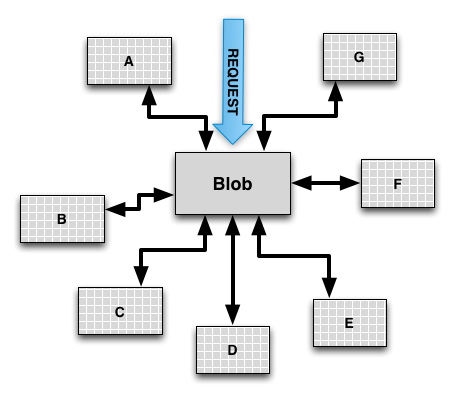
\includegraphics[width=0.8\textwidth]{./images/BLOB.png}
\caption{The God class\cite{Wert2013a}. }
\label{fig:godclass}
\end{minipage}
\end{figure}

Unbalanced Processing it's characterises for one scenario where a specific class of requests generates a pattern of execution within the system that tends to overload a particular resource. In other words the overloaded resource will be executing a certain type of job very often, thus in practice damaging other classes
of jobs that will experience very long waiting times. Unbalanced Processing occurs in three different situations. The first case that cause unbalanced processing it is when processes cannot make effective use of available processors either because processors are dedicated to other tasks or because of single-threaded code. This manifestation has available processors and we need to ensure that the software is able to use them. Fig. \ref{fig:unbalanced}  shows a sample of the Unbalanced Processing. In The Fig. \ref{fig:unbalanced}, four tasks are performed. The task D it is waiting for the task C conclusion that are submmited to a heavy processing situation. 


\begin{figure}[h]
\centering
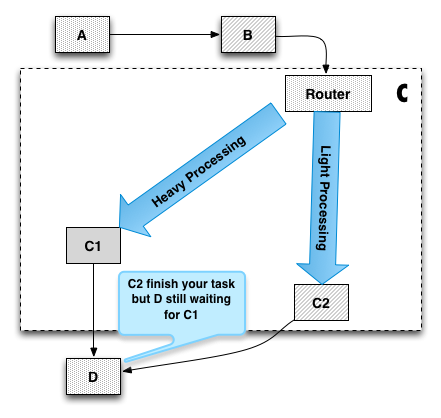
\includegraphics[width=0.4\textwidth]{./images/unbalanced.png}
\caption{Unbalanced Processing sample \cite{Wert2013a}. }
\label{fig:unbalanced}
\end{figure}

Circuitous Treasure Hunt antipattern occurs when software retrieves data from a first componet, uses those results in a second component, retrieves data from the second component, and so on, until the last results are obtained \cite{Smith2002} \cite{Smith2003}. Circuitous Treasure Hunt 
are typical performance antipatterns that causes unnecessarily frequent database requests. The Circuitous Treasure Hunt antipattern is a result from a bad database schema or query design. A common Circuitous Treasure Hunt design creates a data dependency between single queries. For instance, a query requires the
result of a previous query as input. The longer the chain of
dependencies between individual queries the more the Circuitous
Treasure Hunt antipattern hurts performance \cite{Wert2014}. 

The Tower of Babel antipattern most often occurs when information is translated into an exchange format, such as XML, by the sending process then parsed and translated into an
internal format by the receiving process. When the translation and parsing is excessive, the system spends most
of its time doing this and relatively little doing real work \cite{Smith2003}.

\begin{figure}[h]
\begin{minipage}{.5\textwidth}
\centering
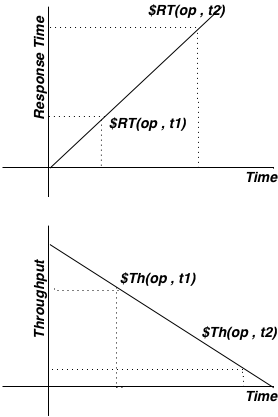
\includegraphics[width=0.5\textwidth]{./images/ramp.png}
\caption{The Ramp sample \cite{Vetoio2011}.}
\label{fig:ramp}
\end{minipage}
\end{figure}

The Ramp it is a antipattern where the processing time increases as the system is used. The Ramp can arise in several different ways. Any situation in which the amount of processing required to satisfy a request increases over time will produce the behavior. With the Ramp antipattern, the memory consumption of the application is growing over time. The root cause is Specific Data Structures which are growing during operation or which are not properly disposed \cite{Wert2014} \cite{Smith2003}. Fig. \ref{fig:ramp} shows a system  with The Ramp problem:  (i) the monitored response time of the operation opx at time t1, i.e. \$RT(opx, t1), is much lower than the monitored response time of the operation opx at time t2, i.e. \$RT(opx, t2), with t1 < t2; (ii) the monitored throughput of the operation opx at time t1, i.e. \$Th(opx, t1), is much larger than the monitored throughput of the operation opx at time t2, i.e. \$Th(opx, t2), with t1 < t2. 

To emulate the presented antipatterns the testbed solution uses Mock Objects with the JMeter load test tool.